%  article.tex (Version 3.3, released 19 January 2008)
%  Article to demonstrate format for SPIE Proceedings

%  The following commands have been added in the SPIE class 
%  file (spie.cls) and will not be understood in other classes:
%  \supit{}, \authorinfo{}, \skiplinehalf, \keywords{}
%  The bibliography style file is called spiebib.bst, 
%  which replaces the standard style unstr.bst.  

%----------------------------------------------------------------------------------------------------
% PACKAGES
%----------------------------------------------------------------------------------------------------

\documentclass[]{spie}  % use for US letter paper
\usepackage{comment}
%%\documentclass[a4paper]{spie}  %>>> use this instead for A4 paper
%%\documentclass[nocompress]{spie}  %>>> to avoid compression of citations
\usepackage[]{graphicx}
\usepackage{epsfig}		% TeX will automatically convert eps --> pdf in pdflatex	
\usepackage{epstopdf}
\usepackage{caption}
\usepackage{subcaption}
\usepackage{multirow}
\usepackage{array}
\usepackage{tabularx}
\usepackage{enumerate}
\usepackage{amsmath}
\usepackage{amsfonts}
\usepackage{bbm}
\usepackage[mathcal]{euscript}
\usepackage{mathtools}

\setcounter{MaxMatrixCols}{14}
\DeclarePairedDelimiter\floor{\lfloor}{\rfloor}
%\renewcommand{\baselinestretch}{1.65}   %>>> 1.65 for double spacing, 1.25 for 1.5 spacing 
%\addtolength{\voffset}{9mm}   %>>> moves text field down

%----------------------------------------------------------------------------------------------------
% TITLE
%----------------------------------------------------------------------------------------------------

\title{An Online Visual Loop Closure Detection Method for Indoor Robotic Navigation} 

%----------------------------------------------------------------------------------------------------
% AUTHORS
%----------------------------------------------------------------------------------------------------

\author{
Can Erhan\supit{a}, 
Evangelos Sariyanidi\supit{b}, 
Onur Sencan\supit{a}, 
Hakan Temeltas\supit{a}
\skiplinehalf
\supit{a}Istanbul Technical University Control and Automation Engineering Department, \\
Maslak 34469, Istanbul, Turkey; \\
\supit{b}Centre of Intelligent Sensing, Mile End Road, E1 4NS, London, U.K.
}

\authorinfo{Further author information: \\
Can Erhan: E-mail: erhanc@itu.edu.tr \\  
Evangelos Sariyanidi: E-mail: e.sariyanidi@eecs.qmul.ac.uk \\
Onur Sencan: E-mail: osencan@itu.edu.tr \\  
Hakan Temeltas: E-mail: hakan.temeltas@itu.edu.tr}
% when using amstex, you need to use @@ instead of @
 
% uncomment following for page numbers
% \pagestyle{plain}    
% uncomment following to start page numbering at 301 
% \setcounter{page}{301} 
 
 %----------------------------------------------------------------------------------------------------
% ABSTRACT
%----------------------------------------------------------------------------------------------------
 
 \begin{document} 
\maketitle 

\begin{abstract}
In this paper, we present an enhanced loop closure method based on image-to-image matching  relies on Quantized Local Zernike Moments. In contradistinction to the previous methods, our approach uses additional depth information to extract Zernike Moments in local manner. These moments are used to represent holistic shape information inside the image. The complex moments that are extracted from both gray and depth images are coarsely quantized. In order to find out the similarity between two locations, Nearest Neighbour classification algorithm is performed. Examplary results and the practical implementation case of the method are also given with the data gathered on the testbed using a Kinect. The method is evaluated in three different datasets of different lighting conditions. Additional depth information beside the actual image increases the detection rate especially in dark. The results are referred as a successful, high-fidelity online method for visual place recognition as well as to close navigation loops, which is a crucial information for the well known Simultaneously Localization and mapping (SLAM) problem. This technique is quite simple because of its low computational complexity, and performs in real-time with high loop closing accuracy.

\end{abstract}

\keywords{Loop closure, Zernike Moments, image processing, SLAM, depth map, indoor navigation}

%----------------------------------------------------------------------------------------------------
% INTRODUCTION
%----------------------------------------------------------------------------------------------------

\section{INTRODUCTION}

In mobile robotics, autonomous navigation is an active research area especially for the indoor environments, where the global position information is missing and the localization information is highly dependent on odometry sensors. One of the major problems linked to robotic navigation is SLAM which still remains as an assertive problem in a lot of ways. Loop closing is defined as the correct identification of previously visited location in terms of SLAM. Information that is gathered from various data sources including LIDARs, RADARs, stereo and monocular cameras\cite{williams08iros, 5650234} is highly utilized in loop closure detection. With the recent development of visual sensor technologies, the loop closure detection became a problem that is open for research in the field of computer vision.

Visual loop closing techniques can be categorized into three main parts\cite{Williams09}: Image-to-image and image-to-map, map-to-map techniques. Loop closure estimations\cite{sariyanidi_spie13}  are cast by matching images. Most of image-to-image techniques that rely on salient image patches, use small, low-level features such as SURF\cite{springerlink:10.1007/11744023_32} extracted from the whole image \cite{sariyanidi_iv, HoNewmanCIRA2005, CumminsNewmanIJRR08}. One of the widely used methods in visual place recognition problem is the Bag of Words\cite{1238663} method. Also, there are some studies that uses additional depth information\cite{kerl2013-IROS} in loop closure problems.More information related to visual loop closing approaches can be found on the relevant survey \cite{Williams09}.

In this paper, we present an enhanced loop closure method based on image-to-image matching with the additional depth information in indoor environments. Specifically, we adopt visual place recognition without using any metrical information such as rotation and exact location to correctly identify the previously visited location. This technique is quite simple because of its low computational complexity, and performs in real-time with high loop closing accuracy. 

The technique we implement relies on discrete Complex Zernike Moments (CZMs) in 2-dimensional space. They are extracted using a set of complex polynomials which form a complete orthogonal radial basis functions defined on the unit disc. These moments are used to represent shape information inside the image within the context of image processing. To make the image description more robust, the ZMs of the input image is calculated in local manner. In this study, the ZMs are extracted from both the greyscale and depth images separately and concatenated sequentially to create ultimate feature vector.

The locations are represented with the histograms of their images. Detecting loop closing events can be considered as a machine learning problem which number of classes expands continuously when a new unseen location comes. We utilized Nearest Neighbour (NN) algorithm to classify locations by which the distance metric is the regular $L_1$ a.k.a. Manhattan distance that is one of the simplest distance metric available. In other words, the image which distance between the input image is minimum closes the loop, if the distance is lower than the predefined threshold value. 

In the following sections, a brief introduction about the methodology is explained first, and then the experiments and datasets are shown, and finally results are presented. 

%----------------------------------------------------------------------------------------------------
% METHODOLOGY
%----------------------------------------------------------------------------------------------------

\section{METHODOLOGY}
\label{sec:method}

As it was mentioned earlier, the presented loop closing approach relies on calculating the Zernike Moments of partitioned image blocks across the input image in a local manner. 

The whole image representation is constructed as follows. Firstly, the ZMs of each subimage that were obtained by partitioning the input image is calculated. After that, the calculated complex moments are coarsely quantized by keeping only the sign of the real and imaginary components and ignoring the rest of the information. Next, the quantized binary data is combined linearly by weighting each of them to convert them into integers. Finally, the integers values are coded as histograms.

%%% PARTITIONED IMAGE
\begin{figure}[!htb]
        \centering
         % trim parameters by order: left, bottom, right, top
        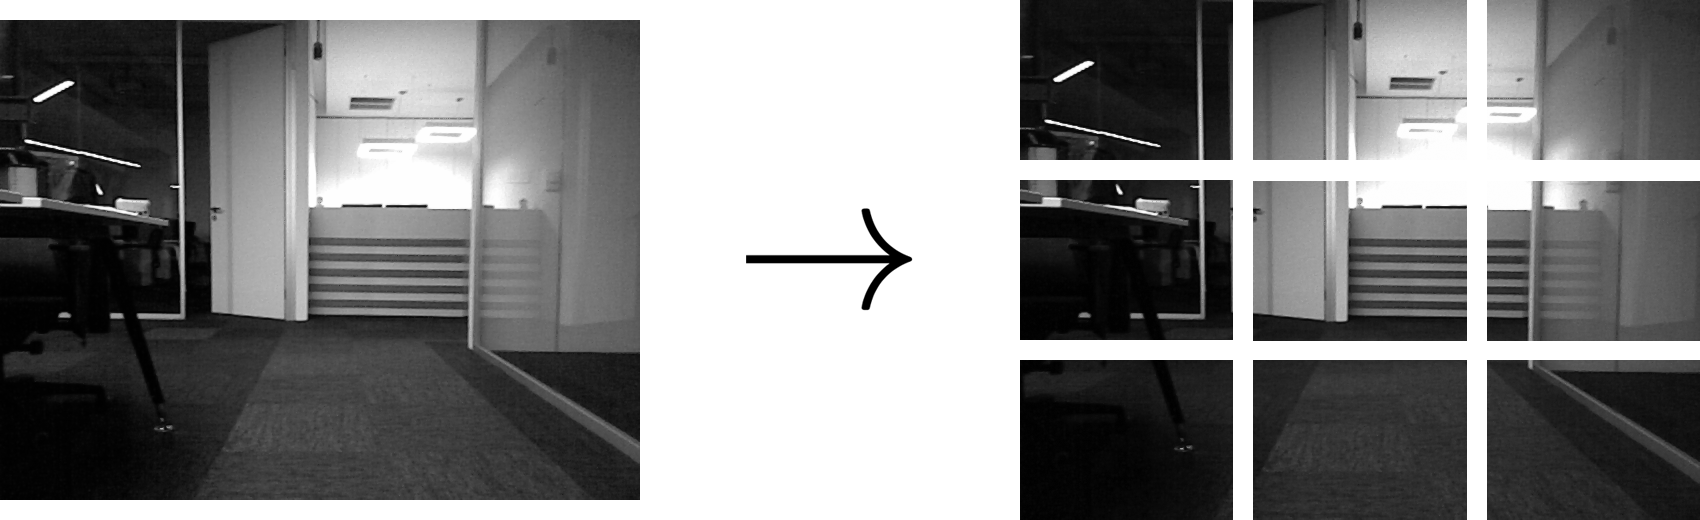
\includegraphics[trim = 0mm 0mm 0mm 0mm, clip, height=3cm]{figures/divided_image.png}    
        \vspace{3mm}
        \caption{Image partitioned into $3\times 3$ blocks ($k = 3$).}
        \label{fig:divided_image}
\end{figure}

\subsection{Extraction of Quantized Local Zernike Moments} 

The Complex Zernike Moments (ZM) of an image are used to represent the image on the 2-dimensional complex subspace. They are extracted using a set of complex polynomials which form a complete orthogonal radial basis functions defined on the unit disc. The coefficients in this complex subspace describe the holistic shape information within the image. 

The Complex Zernike Moments of an image $f(i,j)$ are calculated as follows:

\begin{equation}
\label{eq:global_zernike}
Z_{nm} = \frac{n+1}{\pi}\sum^{N-1}_{i=0}\sum^{N-1}_{j=0}f(i,j)V^\star(\rho_{ij},\theta_{ij})\Delta
x_i\Delta y_j, \\
\end{equation}
where $x_i$, $y_j$ stand for the image coordinates, $\quad\rho_{ij}=\sqrt{x_i^2+y_i^2}$ and $\quad\theta_{ij} = \tan^{-1}\frac{y_j}{x_i}$ are the polar coordinates of the image, $n$ defines the order of the ZM and $m$ stands for the number of repetitions. The constraint between $n$ and $m$ is stated that $|m|\leq n$, and $n-|m|$ must be even. Therefore, the number of components with respect to moment order $n$ is calculated as follows:

\begin{equation}
K(n) =
\begin{cases}
  \frac{n(n+2)}{4} &\text{if $n$ is even} \\ 
  \frac{(n+1)^2}{4} &\text{if $n$ is odd}.
\end{cases}
\label{eq:num_moms}
\end{equation}

In order to extract ZMs in local manner, the input image is divided by $k\times k$-sized subimages in which $k$ is a predefined partitioning parameter. If the image is not divided by $k$ perfectly, the rest of the part is simply ignored. The set of images obtained from partitioning are flatten into a  $k^2\times 1$-sized single column in row-major order for more straightforward representation.

Consider that the input image $\mathbf{I}_{p\times q}$ is a combination of subimages $I_{ij}$:

\begin{equation}
\mathbf{I}_{p\times q} = \begin{bmatrix}
 I_{11} & \hdots & I_{1Q} \\
 \vdots & \ddots & \vdots \\
 I_{P1} & \hdots & I_{PQ} 
 \end{bmatrix}
 \longrightarrow
 \begin{bmatrix}
 I_{11} \\
 \vdots \\
 I_{1Q} \\
 \vdots \\
 I_{P1} \\
 \vdots \\
 I_{PQ}
 \end{bmatrix}
 \label{eq:divided_mat}
\end{equation}
where $P=\floor*{^p/_k}$ and $Q=\floor*{^q/_k}$. An exemplar input image partitioned into subimages is shown in Figure \ref{fig:divided_image}. The $Z_{nm}$ of the input image can be considered as the transformation of the subimages in (\ref{eq:divided_mat}) individually. This transform is applied to subimages with all $n$ and $m$ values according to its order. Lastly, the ZMs computed from transformed subimages are collected into a new matrix as follows:

\begin{equation}
\mathbf{Z} ( \mathbf{I}_{p\times q} )= 
\begin{bmatrix}
\mathbf{Z}(I_{11}) \\
  \vdots \\
\mathbf{Z}(I_{1Q}) \\
  \vdots \\
\mathbf{Z}(I_{P1}) \\
  \vdots \\
\mathbf{Z}(I_{PQ}) \\
 \end{bmatrix}
 \longrightarrow
 \begin{bmatrix}
Z_{00}(I_{11}) & \hdots & Z_{nm}(I_{11}) \\
  \vdots  & & \vdots \\
Z_{00}(I_{1Q}) & \hdots & Z_{nm}(I_{1Q}) \\
  \vdots  & & \vdots \\
Z_{00}(I_{P1}) & \hdots & Z_{nm}(I_{P1}) \\
  \vdots  & & \vdots \\
Z_{00}(I_{PQ}) & \hdots & Z_{nm}(I_{PQ}) \\
 \end{bmatrix} = 
 \begin{bmatrix}
a_{00}^{11} + \mathbf{i}b_{00}^{11} & \hdots & a_{nm}^{11} + \mathbf{i}b_{nm}^{11} \\
  \vdots  & & \vdots \\
a_{00}^{1Q} + \mathbf{i}b_{00}^{1Q} & \hdots & a_{nm}^{1Q} + \mathbf{i}b_{nm}^{1Q} \\
  \vdots  & & \vdots \\
a_{00}^{P1} + \mathbf{i}b_{00}^{P1} & \hdots & a_{nm}^{P1} + \mathbf{i}b_{nm}^{P1} \\
  \vdots  & & \vdots \\
a_{00}^{PQ} + \mathbf{i}b_{00}^{PQ} & \hdots & a_{nm}^{PQ} + \mathbf{i}b_{nm}^{PQ} \\
 \end{bmatrix}.
 \label{eq:lzm_op}
\end{equation}

Therefore, $k^2\times K(n)$-sized complex coefficient matrix is obtained. In order to facilitate the representation of the data and to reduce the size of the descriptor vector, a coarse quantization takes place at this step. First, the complex numbers are decoupled as real and imaginary components, then the sign of each matrix element is taken to binarize the decoupled $k^2\times 2K(n)$-sized matrix as follows:

\begin{equation}
\mathbf{Z} ( \mathbf{I}_{p\times q} )
 \longrightarrow
 \begin{bmatrix}
a_{00}^{11} & b_{00}^{11} & \hdots & a_{nm}^{11}  & b_{nm}^{11} \\
  \vdots  & \vdots & & \vdots  & \vdots\\
a_{00}^{1Q} & b_{00}^{1Q} & \hdots & a_{nm}^{1Q}  & b_{nm}^{1Q} \\
  \vdots  & \vdots & & \vdots  & \vdots\\
a_{00}^{P1} & b_{00}^{P1} & \hdots & a_{nm}^{P1}  & b_{nm}^{P1} \\
  \vdots  & \vdots & & \vdots  & \vdots\\
a_{00}^{PQ} & b_{00}^{PQ} & \hdots & a_{nm}^{PQ}  & b_{nm}^{PQ} \\
 \end{bmatrix}
  \longrightarrow
  \begin{bmatrix}
sgn(a_{00}^{11}) & sgn(b_{00}^{11}) & \hdots & sgn(a_{nm}^{11}) & sgn(b_{nm}^{11}) \\
  \vdots  & \vdots & & \vdots  & \vdots\\
sgn(a_{00}^{1Q}) & sgn(b_{00}^{1Q}) & \hdots & sgn(a_{nm}^{1Q}) & sgn(b_{nm}^{1Q}) \\
  \vdots  & \vdots & & \vdots  & \vdots\\
sgn(a_{00}^{P1}) & sgn(b_{00}^{P1}) & \hdots & sgn(a_{nm}^{P1}) & sgn(b_{nm}^{P1}) \\
  \vdots  & \vdots & & \vdots  & \vdots\\
sgn(a_{00}^{PQ}) & sgn(b_{00}^{PQ}) & \hdots & sgn(a_{nm}^{PQ}) & sgn(b_{nm}^{PQ}) \\
 \end{bmatrix}
 \label{eq:lzm_binary}
\end{equation}
where $sgn(\bullet)$ is the signum function. According to (\ref{eq:global_zernike}), $Z_{nm}$ with $m = 0$ is omitted since their imaginary components turn out to be constantly equal to zero. 

The next step is representing the binary matrix shown in (\ref{eq:lzm_binary}) with histograms. Using the binary values for the overall image representation is not a practical solution. Describing binary data with histograms are more common solution to obtain the image representation. As the methodology described so far, $k^2\times 2K(n)$-sized binary matrix is extracted. Each row of this matrix is linearly combined by weighting each of them as a power of $2$. Hence a column vector $\mathbf{C}$ is obtained with integer values ranging between $0$ and $2^{2K(n)-1}-1$:

\begin{equation}
\mathbf{C} = 
\begin{bmatrix}
c_{j}
\end{bmatrix}=
  \begin{bmatrix}
sgn(a_{00}^{11}) & sgn(b_{00}^{11}) & \hdots & sgn(a_{nm}^{11}) & sgn(b_{nm}^{11}) \\
  \vdots  & \vdots & & \vdots  & \vdots\\
sgn(a_{00}^{1Q}) & sgn(b_{00}^{1Q}) & \hdots & sgn(a_{nm}^{1Q}) & sgn(b_{nm}^{1Q}) \\
  \vdots  & \vdots & & \vdots  & \vdots\\
sgn(a_{00}^{P1}) & sgn(b_{00}^{P1}) & \hdots & sgn(a_{nm}^{P1}) & sgn(b_{nm}^{P1}) \\
  \vdots  & \vdots & & \vdots  & \vdots\\
sgn(a_{00}^{PQ}) &sgn(b_{00}^{PQ}) & \hdots & sgn(a_{nm}^{PQ}) & sgn(b_{nm}^{PQ}) \\
 \end{bmatrix}
 \begin{bmatrix}
2^0 \\
2^1 \\
 \vdots \\
 \vdots \\
 \vdots \\
 2^{2 K(n)-2} \\
 2^{2 K(n)-1}
 \end{bmatrix}
 \label{eq:lzm_coded}
\end{equation}

Finally, the histogram is defined that consists of $2^{2K(n)-1}$ bins, and each bin is filled with the number of occurrences of the integers in $\mathbf{C}$. Therefore, the input image $I_{p\times q}$ is described with a histogram of length of $2^{2K(n)-1}$.

%----------------------------------------------------------------------------------------------------
% EXPERIMENTS
%----------------------------------------------------------------------------------------------------

\section{EXPERIMENTS}

The method implemented in this paper has been evaluated on three datasets which lighting conditions are different from each other. The tests are done with either using gray and depth images separately or using both of them. After that, the difference matrices are calculated to examine the results. Nearest Neighbour (NN) algorithm is applied to classify the new locations using the $L_{1}$ distance metric. In addition to this, the last 100 frames are not included in the classification phase, because it the sensor is always moving and these frames correspond to the area behind the sensor.

The method described in Section \ref{sec:method} has basically two parameters that must be adjusted. One of them is $k\times k$ which defines the number of the subimages that the input image was partitioned to, and the other one is n, which is the order of the Zernike polynomials used. During the experiments, the selected parameters are $k = 30$ and $n = 2$. Then, the quantized $k\times k$-sized matrix obtained from the input image is divided into $5\times 5$ equal-sized non-overlapping subregions. The histograms of each subregion are simply concatenated to compose the feature vector of an image. In order to construct the ultimate feature vector containing both gray and depth images, each feature vector obtained from both images are also concatenated.

\subsection{Benchmark of the Datasets}

In order to measure loop closing performance of the algorithm in different illumination levels, three different datasets are created in an indoor environment by using Kinect sensor which can grab both gray and depth images at the same time. The lighting conditions in the datasets are bright, dim and dark in which both depth and gray images are captured. The exemplary images belonging to different datasets are shown in Figure \ref{fig:dataset}. In some cases, the line of sight of the Kinect is not enough to capture the depth information for distances above $10m$. Thus, some of the depth images are unreliable.

The images in the datasets are acquired via Kinect mounted moving platform and pointed in the direction of the displacement with approximate speed 0.25m/s. Also, the rectangle-shaped trajectory of the three datasets is almost the same as the others to compare their performances correctly. There are two loops that contain around 1000 frames per loop in each dataset, first one is used for discovering and the second for evaluating. To create the ground truth, the locations which corresponds to approximately 10 sequential frames are annotated manually. 

% BENCHMARK DATASETS
\begin{figure}[!htb]
        \centering
        
        %%% BRIGHT 
        \begin{subfigure}[b]{0.27\textwidth}
        \centering
         % trim parameters by order: left, bottom, right, top
        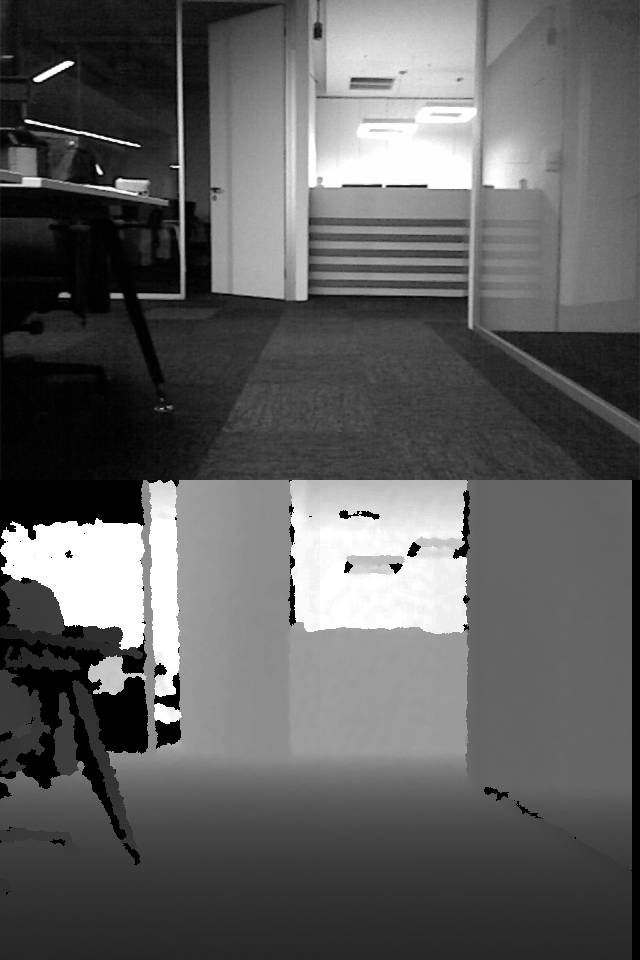
\includegraphics[trim = 0mm 0mm 0mm 0mm, clip, width=\textwidth]{figures/dataset_bright.png}    
        \caption{Bright}
        \label{subfig:dataset_bright}
        \end{subfigure}
        ~ 
        %%% DIM 
        \begin{subfigure}[b]{0.27\textwidth}
        \centering
         % trim parameters by order: left, bottom, right, top
        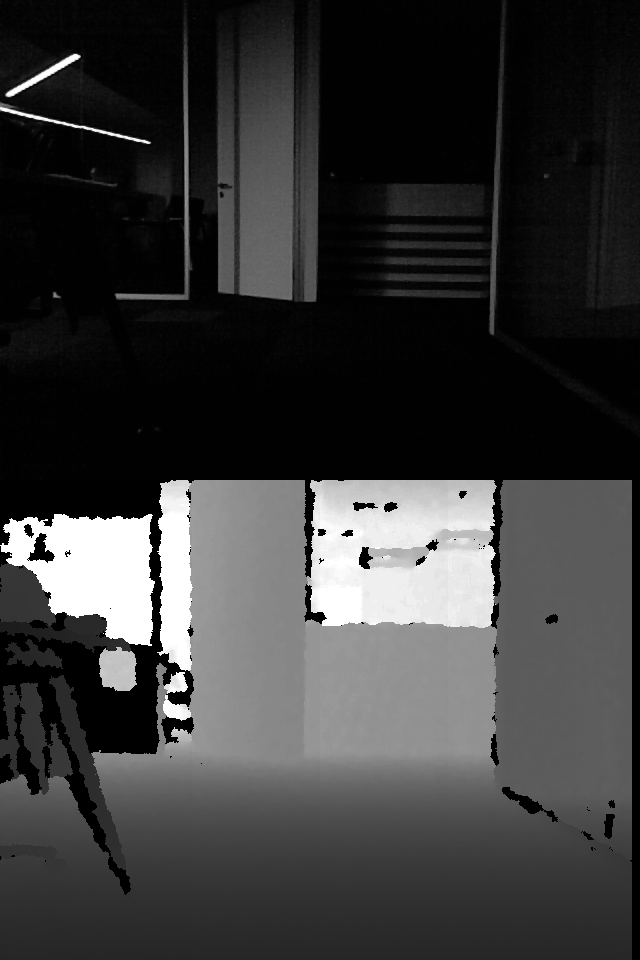
\includegraphics[trim = 0mm 0mm 0mm 0mm, clip, width=\textwidth]{figures/dataset_dim.png}    
        \caption{Dim}
        \label{subfig:dataset_dim}
        \end{subfigure}
         ~ 
        %%% DARK
        \begin{subfigure}[b]{0.27\textwidth}
        \centering
         % trim parameters by order: left, bottom, right, top
        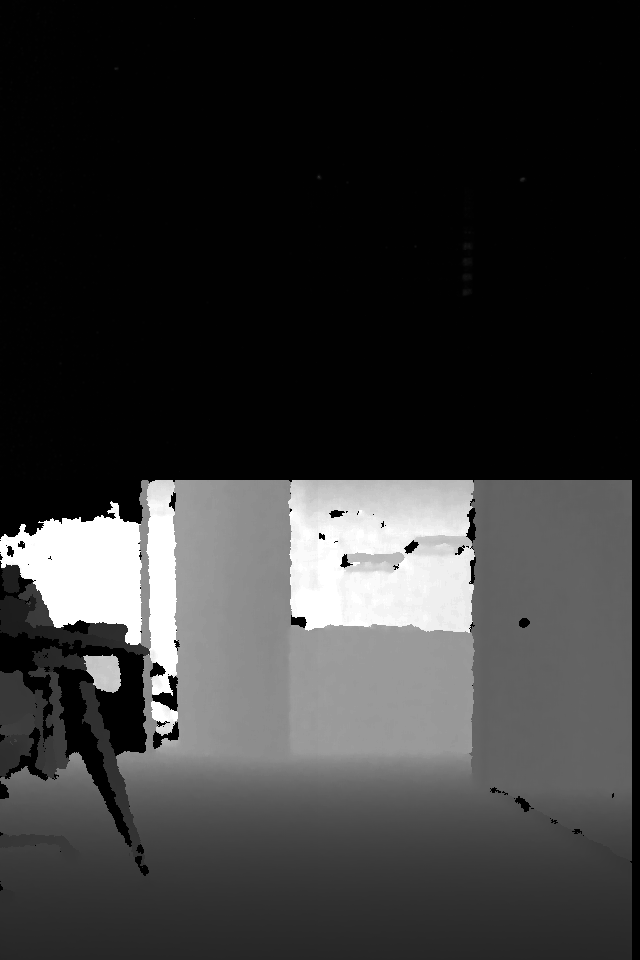
\includegraphics[trim = 0mm 0mm 0mm 0mm, clip, width=\textwidth]{figures/dataset_dark.png}    
        \caption{Dark}
        \label{subfig:dataset_dark}
        \end{subfigure}
        
        \hspace{-3mm}
        \caption{Examplary images belonging to benchmark datasets in three different lighting conditions.}
        \label{fig:dataset}
\end{figure}

%----------------------------------------------------------------------------------------------------
% RESULTS
%----------------------------------------------------------------------------------------------------

\section{RESULTS}
\label{sec:results}

The results are obtained by three datasets in which the trajectory of the Kinect mounted moving platform is similar to each Dataset that is created in different lightning conditions: Bright, Dim and Dark. In the first loop, there are no loop closures to detect. To examine the performance of the method, precision vs. recall (PR) curves are calculated for each dataset. Precision is simply the fraction of retrieved instances that are relevant, while recall is the fraction of relevant instances that are retrieved. In other words, there are less false positives when the precision is high, and less false negatives when the recall is high. In loop closing problem, high precision is needed to decrease localization errors of the moving autonomous vehicle. The PR curves are illustrated in Figures \ref{subfig:pr_bright}, \ref{subfig:pr_dim}, \ref{subfig:pr_dark} in which there are compared three different image source that are only grayscale images, only depth images and both. The results show that using both grayscale and depth images gives the best performance in bright and dim datasets.







%VANGELden
%the performance shown in Table/figure is  representative as the results are obtained with a %manually annotated �.
%our demo video provides qualitative loop closure results which may be considered to be more representative for our method�s performance


\subsection{Detection Performance}

As it can be seen in Figure \ref{subfig:pr_bright}


\subsection{Online Performance}

There exist limited number of techniques that operate in real-time without parallelization. The speed tests are done with a MacBook Pro 7.1 which specifications are Intel Core 2 Duo 2.4 GHz CPU. In this setting, the extraction of Quantized Local Zernike Moments of an image of size $256\times 192$ pixels takes approximately $10ms$. The NN classification is applied with simple brute-force searching in which the algorithmic complexity is $\mathcal{O}(mn)$ that depends on the number of frames to compare with. In other words, the amount of time needed to performs this search increases throughout the trajectory. Therefore, the total processing time including the brute force search is $14ms$ in average when approximately 2000 frames are processed.

% DISTANCE MATRICES
\begin{figure}[!htb]
        \centering
        
        %%% BRIGHT DISTANCE MATRIX
        \begin{subfigure}[b]{0.27\textwidth}
        \centering
         % trim parameters by order: left, bottom, right, top
        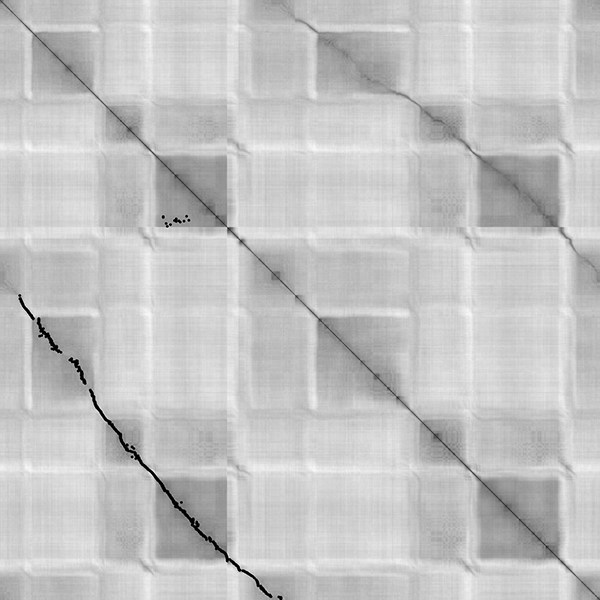
\includegraphics[trim = 0mm 0mm 0mm 0mm, clip, width=\textwidth]{figures/dist_bright.png}    
        \caption{Bright}
        \label{subfig:dist_bright}
        \end{subfigure}
        ~ 
        %%% DIM DISTANCE MATRIX
        \begin{subfigure}[b]{0.27\textwidth}
        \centering
         % trim parameters by order: left, bottom, right, top
        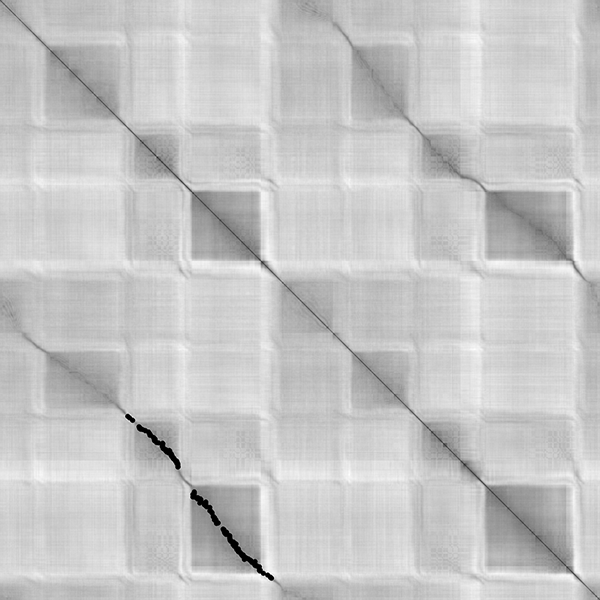
\includegraphics[trim = 0mm 0mm 0mm 0mm, clip, width=\textwidth]{figures/dist_dim.png}    
        \caption{Dim}
        \label{subfig:dist_dim}
        \end{subfigure}
         ~ 
        %%% DARK DISTANCE MATRIX
        \begin{subfigure}[b]{0.27\textwidth}
        \centering
         % trim parameters by order: left, bottom, right, top
        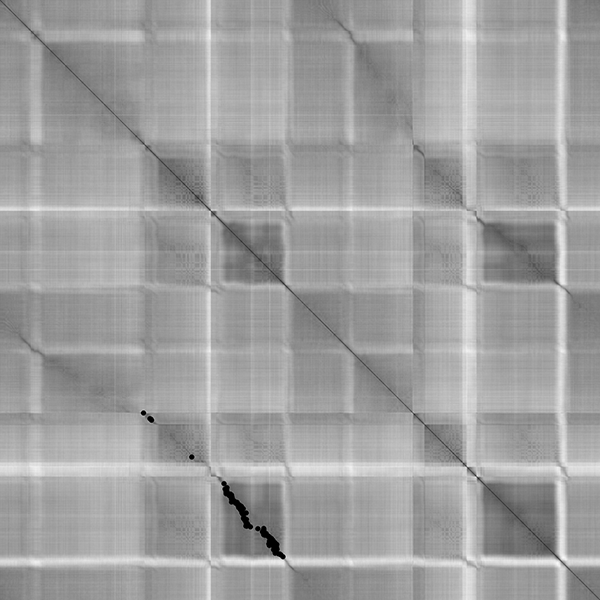
\includegraphics[trim = 0mm 0mm 0mm 0mm, clip, width=\textwidth]{figures/dist_dark.png}    
        \caption{Dark}
        \label{subfig:dist_dark}
        \end{subfigure}
        
        \hspace{-3mm}
        \caption{Similarity matrices of the captured images in experimental results. Condensed gray shades point out to positive alikeness between scenes. The black dots in lower triangle indicates detected loop closures at $90\%$ precision.}
        \label{fig:dist_matrices}
\end{figure}

% RESULTS
\begin{figure}[!htb]
        \centering
        
        %%% BRIGHT PR CURVE
        \begin{subfigure}[b]{0.48\textwidth}
        \centering
         % trim parameters by order: left, bottom, right, top
        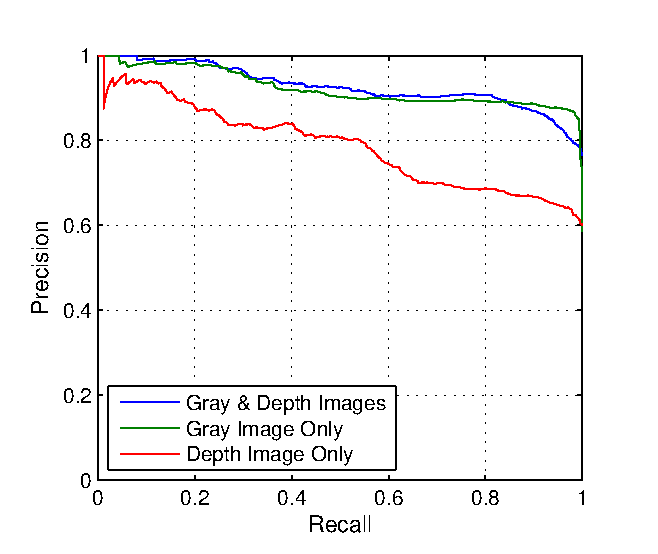
\includegraphics[trim = 0mm 0mm 5mm 0mm, clip, width=\textwidth]{figures/pr_bright.eps}    
        \caption{Bright dataset results.}
        \label{subfig:pr_bright}
        \end{subfigure}
        ~ 
        %%% DIM PR CURVE
        \begin{subfigure}[b]{0.48\textwidth}
        \centering
         % trim parameters by order: left, bottom, right, top
        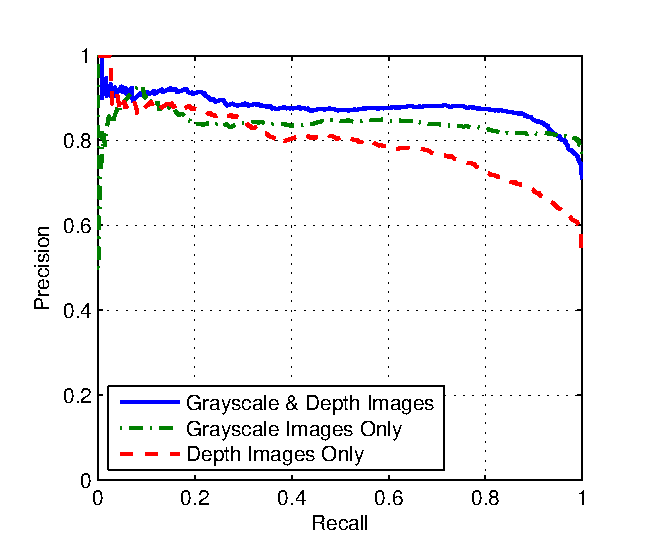
\includegraphics[trim = 0mm 0mm 5mm 0mm, clip, width=\textwidth]{figures/pr_dim.eps}    
        \caption{Dim dataset results.}
        \label{subfig:pr_dim}
        \end{subfigure}
        ~
        %%% DARK PR CURVE
        \begin{subfigure}[b]{0.48\textwidth}
        \centering
         % trim parameters by order: left, bottom, right, top
        \includegraphics[trim = 0mm 0mm 5mm 0mm, clip, width=\textwidth]{figures/pr_dark.eps}    
        \caption{Dark dataset results.}
        \label{subfig:pr_dark}
        \end{subfigure}
        ~ 
        %%% ALL PR CURVE
        \begin{subfigure}[b]{0.48\textwidth}
        \centering
         % trim parameters by order: left, bottom, right, top
        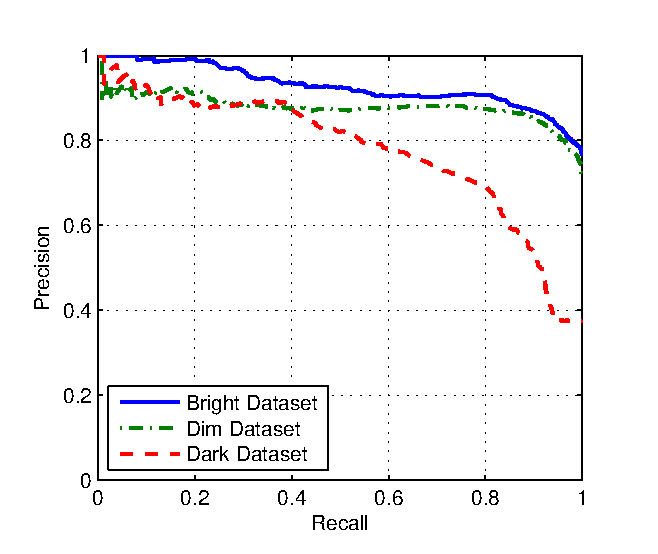
\includegraphics[trim = 0mm 0mm 5mm 0mm, clip, width=\textwidth]{figures/pr_all.eps}    
        \caption{Comparison between datasets.}
        \label{subfig:pr_all}
        \end{subfigure}

        \hspace{-3mm}
        \caption{PR curves}
        \label{fig:pr_curves}
\end{figure}



%----------------------------------------------------------------------------------------------------
% CONCLUSION AND FUTURE WORK
%----------------------------------------------------------------------------------------------------

\section{CONCLUSION AND FUTURE WORK}

%----------------------------------------------------------------------------------------------------
% ACKNOWLEDGEMENTS
%----------------------------------------------------------------------------------------------------

\acknowledgments         

Authors would like to thank for the collaboration and the equipments to ITU Robotics Laboratory and the Borda Technology for the indoor dataset retrieval. 

%----------------------------------------------------------------------------------------------------
% REFERENCES
%----------------------------------------------------------------------------------------------------

\bibliography{report}   % bibliography data in report.bib
\bibliographystyle{spiebib} 

\end{document} 
